\documentclass{amsart}
\usepackage{amsmath}
\usepackage{amssymb}
\usepackage{amsthm}
%\usepackage{MnSymbol}
\usepackage{bm}
\usepackage{accents}
\usepackage{mathtools}
\usepackage{tikz}
\usetikzlibrary{calc}
\usetikzlibrary{decorations.pathmorphing,shapes, decorations.markings}
\usetikzlibrary{automata,positioning, snakes}
\usepackage{tikz-cd}
\usepackage{forest}
\usepackage{braket} 
\usepackage{listings}
\usepackage{mdframed}
\usepackage{verbatim}
\usepackage{physics2}
\usephysicsmodule{ab,ab.legacy,diagmat,xmat, op.legacy}
\usepackage{derivative}
\usepackage{fixdif}
\usepackage{stmaryrd}
% \usepackage{euscript} 
% \usepackage[mathcal]{eucal}
\usepackage{stackengine} 
%\usepackage{/home/patrickl/homework/macaulay2}

%font
\usepackage[sc]{mathpazo}
\usepackage{inconsolata}
\usepackage{microtype}
% \usepackage{fontspec} 
% \setmainfont{Tex Gyre Pagella}
\usepackage[OT1,euler-digits]{eulervm}
% \usepackage{euler-math} 
\usepackage[scaled=0.86]{berasans}
% \let\sffamilyold\sffamily
% \def\sffamily{\fontencoding{T1}\sffamilyold}
% \setmonofont{Inconsolatazi4}

%CS packages
\usepackage{algorithmicx}
\usepackage{algpseudocode}
\usepackage{algorithm}

% typeset and bib
\usepackage[english]{babel} 
% \usepackage[utf8]{inputenc} 
% \usepackage[T1]{fontenc}
% \usepackage[backend=biber,style=alphabetic,maxalphanames=4,maxnames=5,hyperref]{biblatex}
\usepackage[bookmarks, colorlinks, breaklinks]{hyperref} 
\hypersetup{linkcolor=blue,citecolor=magenta,filecolor=black,urlcolor=blue}
\usepackage{cleveref}
\usepackage{graphicx}
\graphicspath{{./}}


% other formatting packages
\usepackage{float}
\usepackage{booktabs}
\usepackage[shortlabels]{enumitem}
\setitemize{noitemsep}
\usepackage{csquotes}
%\usepackage{titlesec}
%\usepackage{titling}
%\usepackage{fancyhdr}
%\usepackage{lastpage}
% \usepackage{parskip}
\newlist{mydescription}{description}{1}
\setlist[mydescription]{style=nextline,
                        font=\bfseries,
                        % Tweak the next 4 options as needed:
                        labelindent=1cm, 
                        leftmargin =2cm,
                        rightmargin=1cm,
                        topsep     =1ex
                       }

\usepackage{lipsum}

% delimiters
\DeclarePairedDelimiter{\gen}{\langle}{\rangle}
\DeclarePairedDelimiter{\floor}{\lfloor}{\rfloor}
\DeclarePairedDelimiter{\ceil}{\lceil}{\rceil}


\newtheorem{thm}{Theorem}[section]
\newtheorem{cor}[thm]{Corollary}
\newtheorem{prop}[thm]{Proposition}
\newtheorem{lem}[thm]{Lemma}
\newtheorem{conj}[thm]{Conjecture}
\newtheorem{quest}[thm]{Question}
\newtheorem{claim}[thm]{Claim}

\theoremstyle{definition}
\newtheorem{defn}[thm]{Definition}
\newtheorem{defns}[thm]{Definitions}
\newtheorem{con}[thm]{Construction}
\newtheorem{exm}[thm]{Example}
\newtheorem{exms}[thm]{Examples}
\newtheorem{notn}[thm]{Notation}
\newtheorem{notns}[thm]{Notations}
\newtheorem{addm}[thm]{Addendum}
\newtheorem{exer}[thm]{Exercise}

\theoremstyle{remark}
\newtheorem{rmk}[thm]{Remark}
\newtheorem{rmks}[thm]{Remarks}
\newtheorem{warn}[thm]{Warning}
\newtheorem{sch}[thm]{Scholium}


% unnumbered theorems
\theoremstyle{plain}
\newtheorem*{thm*}{Theorem}
\newtheorem*{prop*}{Proposition}
\newtheorem*{lem*}{Lemma}
\newtheorem*{cor*}{Corollary}
\newtheorem*{conj*}{Conjecture}

% unnumbered definitions
\theoremstyle{definition}
\newtheorem*{defn*}{Definition}
\newtheorem*{exer*}{Exercise}
\newtheorem*{defns*}{Definitions}
\newtheorem*{con*}{Construction}
\newtheorem*{exm*}{Example}
\newtheorem*{exms*}{Examples}
\newtheorem*{notn*}{Notation}
\newtheorem*{notns*}{Notations}
\newtheorem*{addm*}{Addendum}


\theoremstyle{remark}
\newtheorem*{rmk*}{Remark}

% shortcuts
\newcommand{\Ima}{\mathrm{Im}}
\newcommand{\A}{\mathbb{A}}
\newcommand{\G}{\mathbb{G}}
\newcommand{\N}{\mathbb{N}}
\newcommand{\R}{\mathbb{R}}
\newcommand{\C}{\mathbb{C}}
\newcommand{\Z}{\mathbb{Z}}
\newcommand{\Q}{\mathbb{Q}}
\newcommand{\E}{\mathbb{E}}
\renewcommand{\k}{\Bbbk}
\renewcommand{\L}{\mathbb{L}}
\renewcommand{\P}{\mathbb{P}}
\newcommand{\M}{\mathcal{M}}
\newcommand{\Mbar}{\overline{\mathcal{M}}}
\newcommand{\g}{\mathfrak{g}}
\newcommand{\h}{\mathfrak{h}}
\newcommand{\n}{\mathfrak{n}}
\renewcommand{\b}{\mathfrak{b}}
\newcommand{\ep}{\varepsilon}
\newcommand*{\dt}[1]{%
   \accentset{\mbox{\Huge\bfseries .}}{#1}}
%\renewcommand{\abstractname}{Official Description}
\newcommand{\mc}[1]{\mathcal{#1}}
% \newcommand{\msc}[1]{\mathscr{#1}}
\newcommand{\T}{\mathbb{T}}
\newcommand{\mf}[1]{\mathfrak{#1}}
\newcommand{\mbf}[1]{\mathbf{#1}}
\newcommand{\bv}{\mbf{v}}
\newcommand{\bq}{\mbf{q}}
\newcommand{\bp}{\mbf{p}}
\newcommand{\btau}{\bm{\tau}}
\newcommand{\mr}[1]{\mathrm{#1}}
\newcommand{\on}[1]{\operatorname{#1}}
\newcommand{\ms}[1]{\mathsf{#1}}
\newcommand{\mt}[1]{\mathtt{#1}}
\newcommand{\ol}[1]{\overline{#1}}
\newcommand{\ul}[1]{\underline{#1}}
\newcommand{\wt}[1]{\widetilde{#1}}
\newcommand{\wh}[1]{\widehat{#1}}
\renewcommand{\div}{\operatorname{div}}
\newcommand{\1}{\mathbf{1}}
\newcommand{\2}{\mathbf{2}}
\newcommand{\3}{\mathbf{3}}
\newcommand{\I}{\mathrm{I}}
\newcommand{\II}{\mr{I}\hspace{-1.3pt}\mr{I}}
\newcommand{\III}{\mr{I}\hspace{-1.3pt}\mr{I}\hspace{-1.3pt}\mr{I}}
\renewcommand{\v}{\mbf{v}}
\newcommand{\w}{\mbf{w}}
\newcommand{\bmu}{\bm{\mu}}
\newcommand{\pre}{\mr{pre}}
\newcommand{\vir}{\mr{vir}}
\newcommand{\fl}{\mr{fl}}
\newcommand{\ps}[1]{\llbracket #1 \rrbracket}
\newcommand{\ls}[1]{\llparenthesis #1 \rrparenthesis}

\DeclareMathOperator{\Der}{Der}
\DeclareMathOperator{\Tor}{Tor}
\DeclareMathOperator{\Hom}{Hom}
\DeclareMathOperator{\End}{End}
\DeclareMathOperator{\Ext}{Ext}
\DeclareMathOperator{\ad}{ad}
\DeclareMathOperator{\Aut}{Aut}
\DeclareMathOperator{\Rad}{Rad}
\DeclareMathOperator{\Pic}{Pic}
\DeclareMathOperator{\NS}{NS}
\DeclareMathOperator{\supp}{supp}
\DeclareMathOperator{\Supp}{Supp}
\DeclareMathOperator{\depth}{depth}
\DeclareMathOperator{\sgn}{sgn}
\DeclareMathOperator{\spec}{Spec}
\DeclareMathOperator{\Spec}{Spec}
\DeclareMathOperator{\proj}{Proj}
\DeclareMathOperator{\Proj}{Proj}
\DeclareMathOperator{\ord}{ord}
\DeclareMathOperator{\Div}{Div}
\DeclareMathOperator{\Bl}{Bl}
\DeclareMathOperator{\coker}{coker}
\DeclareMathOperator{\ev}{ev}
\DeclareMathOperator{\st}{st}
\DeclareMathOperator{\pr}{pr}
\DeclareMathOperator{\ch}{ch}
\DeclareMathOperator{\Cont}{Cont}

% \addbibresource{../../notes/math.bib}

\title{Good moduli spaces, positivity and rationality}
\author{Lectures by Maksym Fedorchuk \\ Notes by Patrick Lei}
\date{Spring 2026}
\allowdisplaybreaks

\begin{document}
    
\begin{abstract}
    This course will be an introduction to the theory of good moduli
spaces (in the sense of Alper). We will generalize filtrations from a
vector space to an algebraic variety, define theta-reductivity,
S-completeness, and unpuncturedness of inertia. Examples will include
good moduli spaces for Deligne-Mumford stable curves, and K-semistable
Fanos, with the focus on the cases where there is a positive
tautological line bundle and the good moduli space is particularly
simple, i.e., rational.
\end{abstract}

\maketitle

\tableofcontents

\section{Moduli of rational curves}%
\label{sec:Moduli of rational curves}

We will begin by interpolating between $\ol{M}_{0,n}$ (which is a scheme) and the stack $(\P^1)^n \sslash \on{PGL}(2)$ (which has a good moduli space by definition) via Hassett spaces $\ol{M}_{0, A}$. There is a single smooth rational curve, which is $\P^1 = \ab\{x = 0\} \subseteq \P^2_{x,y,z}$.

Viewing the curve inside $\P^2$, we may (see~\Cref{fig:family}) consider the family
\begin{equation*}
\begin{tikzcd}
    \ar[equals]{r} \ab\{xy - t^2 z^2 = 0\} & \mf{X} \ar[hookrightarrow]{r} \ar{d} & \P^2 \\
    & \A^1_t
\end{tikzcd}
\end{equation*}
\begin{figure}[htpb]
\begin{center}
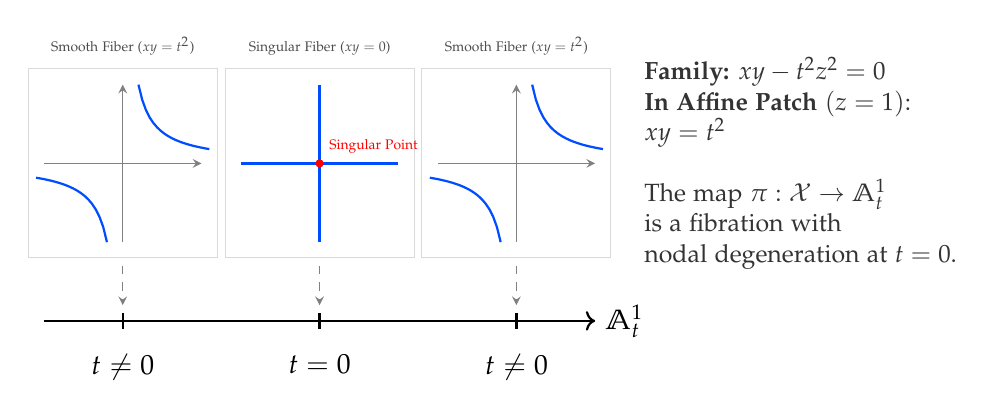
\begin{tikzpicture}[
    scale=1,
    % Define styles for consistency
    axis/.style={->, >=stealth, thin, gray},
    curve/.style={thick, color=blue!70!cyan},
    plane/.style={fill=white, draw=gray!30, fill opacity=0.8},
    fiber_label/.style={font=\footnotesize, text=black!70},
    map_arrow/.style={->, >=stealth, dashed, color=gray}
]

    % ---------------------------------------------------------
    % 1. The Base Line (Affine Line A^1_t)
    % ---------------------------------------------------------
    \draw[thick, ->] (-3.5, -2) -- (3.5, -2) node[right] {$\mathbb{A}^1_t$};
    
    % Ticks on the t-axis
    \foreach \x/\label in {-2.5/$t \neq 0$, 0/$t = 0$, 2.5/$t \neq 0$} {
        \draw[thick] (\x, -2.1) -- (\x, -1.9);
        \node[below, yshift=-3mm] at (\x, -2) {\label};
    }

    % ---------------------------------------------------------
    % 2. The Fibers (The curves in P^2)
    % ---------------------------------------------------------
    % We represent the projective plane P^2 via the affine patch z=1 (a square box)
    
    % --- Fiber 1: t < 0 (Hyperbola) ---
    \begin{scope}[shift={(-2.5, 0)}]
        % Draw Plane Background
        \filldraw[plane] (-1.2, -1.2) rectangle (1.2, 1.2);
        \node[fiber_label, above, font=\tiny] at (0, 1.25) {Smooth Fiber ($xy = t^2$)};
        
        % Axes (for reference)
        \draw[axis] (-1, 0) -- (1, 0);
        \draw[axis] (0, -1) -- (0, 1);
        
        % Hyperbola xy = const (const > 0 since t^2 > 0)
        \draw[curve, domain=0.2:1.1, samples=20] plot (\x, {0.2/\x});
        \draw[curve, domain=0.2:1.1, samples=20] plot (-\x, {-0.2/\x});
        
        % Projection Arrow
        \draw[map_arrow] (0, -1.3) -- (0, -1.8);
    \end{scope}

     % --- Fiber 3: t > 0 (Hyperbola) ---
    \begin{scope}[shift={(2.5, 0)}]
        % Draw Plane Background
        \filldraw[plane] (-1.2, -1.2) rectangle (1.2, 1.2);
        \node[fiber_label, above, font=\tiny] at (0, 1.25) {Smooth Fiber ($xy = t^2$)};

        % Axes (for reference)
        \draw[axis] (-1, 0) -- (1, 0);
        \draw[axis] (0, -1) -- (0, 1);
        
        % Hyperbola xy = const
        \draw[curve, domain=0.2:1.1, samples=20] plot (\x, {0.2/\x});
        \draw[curve, domain=0.2:1.1, samples=20] plot (-\x, {-0.2/\x});

        % Projection Arrow
        \draw[map_arrow] (0, -1.3) -- (0, -1.8);
    \end{scope}

    % --- Fiber 2: t = 0 (Singular Union of Lines) ---
    \begin{scope}[shift={(0, 0)}]
        % Draw Plane Background
        \filldraw[plane] (-1.2, -1.2) rectangle (1.2, 1.2);
        \node[fiber_label, above, font=\tiny] at (0, 1.25) {Singular Fiber ($xy = 0$)};
        
        % Axes ARE the curve here
        \draw[curve] (-1, 0) -- (1, 0); % y=0
        \draw[curve] (0, -1) -- (0, 1); % x=0
        
        % Node point
        \fill[red] (0,0) circle (1.5pt) node[anchor=south west, font=\tiny, color=red] {Singular Point};

        % Projection Arrow
        \draw[map_arrow] (0, -1.3) -- (0, -1.8);
    \end{scope}

   

    % ---------------------------------------------------------
    % 3. Annotations
    % ---------------------------------------------------------
    \node[right, font=\small, align=left, color=black!80] at (4, 0) {
        \textbf{Family:} $xy - t^2z^2 = 0$ \\
        \textbf{In Affine Patch} $(z=1)$: \\
        $xy = t^2$ \\
        \\
        The map $\pi: \mathcal{X} \to \mathbb{A}^1_t$ \\
        is a fibration with \\
        nodal degeneration at $t=0$.
    };
\end{tikzpicture}
\end{center}
\caption{The family \(\ab\{xy - t^2z^2 = 0\}\) over $\A^1$}%
\label{fig:family}
\end{figure}

This morphism is a (flat) isotrivial degeneration, and will be the first example of a test configuration. What this means is that there is an action of $\G_m$ on $\mf{X}$ by the formula
\[ \lambda ([x,y,z],t) = ([\lambda x, \lambda y, z], \lambda t) \]
such that $\mf{X} \to \A^1$ is equivariant. More generally, any tree of rational curves joined by nodes is also a rational curve (as in it has genus $0$). 

\begin{rmk}
    A \textbf{reduced} rational curve is a ``tree'' of $\P^1$'s meeting in $m$-fold rational points, where each singularity is locally analytically isomorphic to the union of the coordinate axes in $\A^m$.

    In fact, the definition of a rational curve tells about what kinds of singularities it has, and then there is a classification of curve singularities. Another viewpoint is that if we degenerate a rational normal curve in $\P^m$ to a cone over a hyperplace section, we get a union of $m$ lines meeting at a point in exactly the way described above.
\end{rmk}

We will now consider the functor $\wt{\mc{U}}_{0,n}$ of $n$-pointed smooth rational curves. In particular, a family $\mf{X} \to B$ must have $n$ sections $\sigma_1, \ldots, \sigma_n \colon B \to \mf{X}$, which are not required to be disjoint. We may now consider the larger functor $\wt{\mc{M}}_{0,n}$ of $n$-pointed reduced rational curves with sections $\sigma_i$ avoiding the singularities of the fibers. Unfortunately, this is extremely non-separated, so we will consider stability conditions.

Define the functor $\ol{M}_{0,n}$ of $n$-pointed rational curves with at worst nodal singularities such that all sections $\sigma_i(B)$ are disjoint and tha4t the relative dualizing sheaf 
\[ \omega_{\mf{X}/B}(\sigma_1 + \cdots + \sigma_n)\]
is relatively ample over $B$. One reason we consider this (and that it makes sense) is that the $m$-fold rational point is Gorenstein if and only if $m \leq 2$. This stability condition was introduced by Deligne and Mumford. In fact, the condition on the relative dualizing sheaf is equivalent to enforcing that the automorphism group of each fiber is finite, but is easier to modify for obvious reasons. From either perspective, it is clear that we must have a tree of $\P^1$'s with at least three special points on each component. One example can be seen in~\Cref{fig:m07bar}.

\begin{figure}[htpb]
\begin{center}
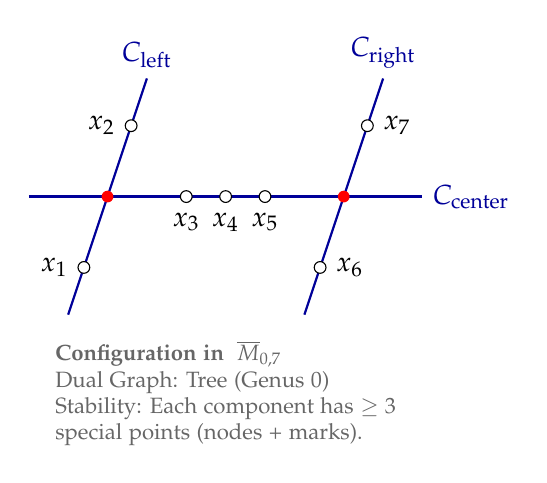
\begin{tikzpicture}[scale=1]
    % Define styles
    \tikzstyle{component}=[thick, color=blue!60!black]
    \tikzstyle{markpoint}=[draw, circle, fill=white, inner sep=1.5pt]
    \tikzstyle{node_singularity}=[fill=red, circle, inner sep=1.5pt]
    \tikzstyle{label_text}=[font=\footnotesize, color=gray!80!black]

    % --- 1. Draw the Components (Lines representing P^1) ---
    
    % Central Component (C_0)
    \draw[component] (-2.5, 0) -- (2.5, 0) node[right] {$C_{\text{center}}$};
    
    % Left Component (C_L) - Intersects at (-1.5, 0)
    \draw[component] (-2, -1.5) -- (-1, 1.5) node[above] {$C_{\text{left}}$};
    
    % Right Component (C_R) - Intersects at (1.5, 0)
    \draw[component] (1, -1.5) -- (2, 1.5) node[above] {$C_{\text{right}}$};

    % --- 2. Draw the Nodes (Intersections) ---
    \node[node_singularity] at (-1.5, 0) {};
    \node[node_singularity] at (1.5, 0) {};

    % --- 3. Draw the Marked Points (x1 to x7) ---
    
    % Points on Left Component (Need 2 marks + 1 node >= 3)
    \node[markpoint, label=left:$x_1$] at (-1.8, -0.9) {};
    \node[markpoint, label=left:$x_2$] at (-1.2, 0.9) {};
    
    % Points on Center Component (Need 3 marks + 2 nodes >= 3)
    \node[markpoint, label=below:$x_3$] at (-0.5, 0) {};
    \node[markpoint, label=below:$x_4$] at (0, 0) {};
    \node[markpoint, label=below:$x_5$] at (0.5, 0) {};
    
    % Points on Right Component (Need 2 marks + 1 node >= 3)
    \node[markpoint, label=right:$x_6$] at (1.2, -0.9) {};
    \node[markpoint, label=right:$x_7$] at (1.8, 0.9) {};

    % --- 4. Annotations ---
    \node[label_text, align=left] at (0, -2.5) {
        \textbf{Configuration in } $\overline{M}_{0,7}$ \\
        Dual Graph: Tree (Genus 0) \\
        Stability: Each component has $\ge 3$ \\
        special points (nodes + marks).
    };

\end{tikzpicture}
\end{center}
\caption{An example of a stable curve of genus $0$ with marked points}%
\label{fig:m07bar}
\end{figure}

One way to turn a family with an $m$-fold rational point into a nodal one is to blow up the singular point. The remaining conditions are non-disjoint sections, which can be separated by finitely many blowups. Finally, the unstable components can be contracted by the basic theory of surfaces (they have self-intersection either $-1$ or $-2$). In particular, we have sketched a proof that $\ol{M}_{0,n}$ is universally closed. In fact, it is also separated, but we will omit the proof here.

Suppose we have a family $\pi \colon \mf{X} \to B$ in $\wt{\mc{M}}_{0,n}$. Then we have $n+1$ line bundles on $B$ where $n$ of them are given by 
\[ \sigma_i^* \omega_{\mf{X}/B} = \sigma_i^*(N_{\sigma_i(B)/X}^{\vee}) \]
(this is fine even in the non-Gorenstein case because the sections avoid the singularities) and the last is given by
\[ \delta = \pi_* (c_2 (\Omega^1_{\mf{X}/B})), \]
which counts singularities. For example, if $B$ is a smooth projective curve, then
\[ \deg \delta = \sum_m m \cdot (\# \ab\{ \text{m-fold singularities} \}). \]

\begin{thm}
    The line bundle
    \[ \psi - \delta = \ab[\sum_{i=1}^n \psi_i] - \delta \]
    is ample on $\ol{M}_{0,n}$.
\end{thm}

\begin{rmk}
    Projectivity of $\ol{M}_{0,n}$ can be proved in more synthetic ways, for example via the explicit blowup construction of Keel.
\end{rmk}

\subsection{Hassett moduli spaces}%
\label{sub:Hassett moduli spaces}

There is a modification of this, which is the functor $\ol{M}_{0, A}$, where
\[ A = (\alpha_1, \ldots, \alpha_n) \in (0,1] \cap \Q. \]
Here, we consider $n$-pointed rational curves which are at worst nodal, but where the sections $\sigma_{i_1}, \ldots, \sigma_{i_k}$ can meet if and only if
\[ \alpha_{i_1} + \cdots + \alpha_{i_k} \leq 1 \]
and the condition on the dualizing sheaf is that $\omega_{\mf{X}/B} \ab( \sum_i \alpha_i \sigma_i)$ is ample. Projectivity of this is proven using similar methods to $\ol{M}_{0,n}$.

More specifically, the functor is given by
\[ \ol{M}_{0, A}(T) = \ab\{ \begin{tikzcd}
    \mc{C} \ar[bend left=20, swap]{d}{\pi} \\ T \ar[bend right = 20, swap]{u}{\sigma_1, \ldots, \sigma_n} \end{tikzcd}
    \middle\vert \Centerstack{{fibers at worst nodal} {$\omega_{\mc{C}/T}\ab(\sum \alpha_i \sigma_i)$ is $\pi$-ample} {sections with sum of weights $>1$ cannot meet}}
 \}. \]
This functor is actually representable by a scheme because the three conditions imply that there are no automorphisms.

\begin{exm}
    If $A = (1, \ldots, 1)$ or more generally if the sum of any two weights is strictly greater than $1$, then $\ol{M}_{0, A} = \ol{M}_{0,n}$.
\end{exm}

\begin{exm}
    If $A = (1, \ep, \ldots, \ep)$ such that $1-(n-1)\ep > 2$ and $\ep \leq \frac{1}{n-2}$, then the combinatorics imply that all marked points lie on the same component. If we call the heavy marked point $\infty$, then all of the light markings lie in $\A^1$. By translation invariance, we may assume that
    \[ x_1 + \cdots + x_{n-1} = 0, \]
    and therefore we obtain 
    \[ [x_1 : \cdots : x_{n-1}] \in \C^{n-2} \setminus \ab\{0\} / \C^{\times} \simeq \P^{n-3}. \]
\end{exm}

\begin{rmk}
    There exists a morphism $\ol{M}_{0,n} \to \ol{M}_{0, A}$ given (when the base is a curve) by changing the weights and contracting all of the $(-1)$-curves in the fibers where the total weight of the sections has weight at most $1$.
\end{rmk}

\begin{exm}
    If we set $A = (\ep, \ldots, \ep)$ such that $\ep \approx \frac{2}{n} + \ep'$, then the curve must be a $\P^1$ with $n$ points such that we cannot have $\ceil{\frac{2}{n}}$ colliding. More concretely, if $n = 2m+1$ and $\ep = \frac{1}{m}$, then we have a $\P^1$ with $2m+1$ marked points such that at most $m$ can collide. In particular, we have
    \begin{align*}
        \ol{M}_{0, A} &= \frac{(\P^1)^{2m+1} \setminus \ab\{ \text{$(m+1)$-fold diagonals} \}}{\on{PGL}(2)} \\
        &= ((\P^1)^{2m+1})^{\mr{ss}} \sslash \on{PGL}(2),
    \end{align*}
    where the linearization is the tensor product of the $\mc{O}(1)$ on each factor. For an example when $m = 7$, see~\Cref{fig:m07weighted}.
    \begin{figure}[htpb]
    \begin{center}
    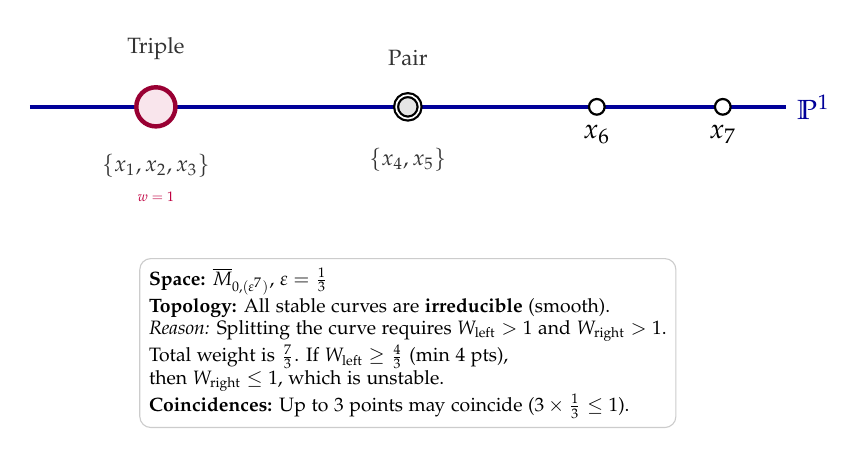
\begin{tikzpicture}[scale=1.6]
    % --- Styles ---
    \tikzstyle{component}=[ultra thick, color=blue!60!black]
    
    % Single Point (w=0.3)
    \tikzstyle{single}=[draw=black, circle, fill=white, inner sep=2pt, thick]
    
    % Pair (w=0.6) - Allowed since 0.6 <= 1
    \tikzstyle{pair}=[draw=black, double, circle, fill=gray!20, inner sep=3pt, thick]
    
    % Triple (w=0.9) - Allowed since 0.9 <= 1 - Draw as a hexagon or larger circle
    \tikzstyle{triple}=[draw=purple!80!black, ultra thick, circle, fill=purple!10, inner sep=5pt]
    
    \tikzstyle{label_text}=[font=\footnotesize, color=black!80]
    \tikzstyle{anno_box}=[draw=gray!40, fill=white, rounded corners, align=left, font=\scriptsize]

    % --- 1. Draw the Component (Irreducible P^1) ---
    \draw[component] (-3, 0) -- (3, 0) node[right] {$\mathbb{P}^1$};

    % --- 2. Draw Marked Points ---
    
    % Triple Coincidence {x1, x2, x3}
    \node[triple] (t1) at (-2, 0) {};
    \node[label_text, above] at (-2, 0.3) {Triple};
    \node[label_text, below] at (-2, -0.3) {$\{x_1, x_2, x_3\}$};
    \node[font=\tiny, color=purple, below] at (-2, -0.6) {$w=1$};

    % Pair Coincidence {x4, x5}
    \node[pair] (p1) at (0, 0) {};
    \node[label_text, above] at (0, 0.25) {Pair};
    \node[label_text, below] at (0, -0.25) {$\{x_4, x_5\}$};

    % Single Points x6, x7
    \node[single, label=below:$x_6$] at (1.5, 0) {};
    \node[single, label=below:$x_7$] at (2.5, 0) {};


    % --- 3. Mathematical Explanation Box ---
    \node[anno_box, anchor=north] at (0, -1.2) {
        \textbf{Space:} $\overline{M}_{0,(\ep^7)}$, $\ep = \frac{1}{3}$ \\
        \textbf{Topology:} All stable curves are \textbf{irreducible} (smooth). \\
        \textit{Reason:} Splitting the curve requires $W_{\text{left}} > 1$ and $W_{\text{right}} > 1$. \\
        Total weight is $\frac{7}{3}$. If $W_{\text{left}} \ge \frac{4}{3}$ (min 4 pts), \\
        then $W_{\text{right}} \le 1$, which is unstable. \\
        \textbf{Coincidences:} Up to 3 points may coincide ($3 \times \frac{1}{3} \le 1$).
    };

\end{tikzpicture}
    \end{center}
    \caption{An object in $\ol{M}_{0, \ab(\frac{3}{10}, \frac{3}{10}, \frac{3}{10}, \frac{3}{10}, \frac{3}{10}, \frac{3}{10}, \frac{3}{10})}$}%
    \label{fig:m07weighted}
    \end{figure}
    
\end{exm}

\subsection{Semistable objects}%
\label{sub:Semistable objects}

Now we will define a new moduli space
\[ \ol{M}_{0, A}^*(T) = \ab\{ \begin{tikzcd}
    \mc{C} \ar[bend right=20, swap]{d}{\pi} \\ T \ar[bend right = 20, swap]{u}{\sigma_1, \ldots, \sigma_n} \end{tikzcd}
    \middle\vert \Centerstack{{fibers at worst nodal} {$\omega_{\mc{C}/T}\ab(\sum \alpha_i \sigma_i)$ is $\pi$-nef} {sections with sum of weights $>1$ cannot meet}}
 \} \]
by relaxing the ampleness condition. This can happen if we have sections whose weights sum to exactly $1$.

\begin{exm}
    If $n = 2m$ and $A = \ab(\frac{1}{m}, \ldots, \frac{1}{m})$, then we have
    \[ \ol{M}_{0, A}^* = (\P^1)^{2m} \sslash \on{PGL}(2). \]
    This is not a scheme and does not even have a coarse moduli space because the curve where the first $m$ markings collide and the last $m$ markings collide has an entire $\G_m$ of automorphisms. For an example when $n=4$, see~\Cref{fig:semistablecurve}.
    \begin{figure}[htpb]
    \begin{center}
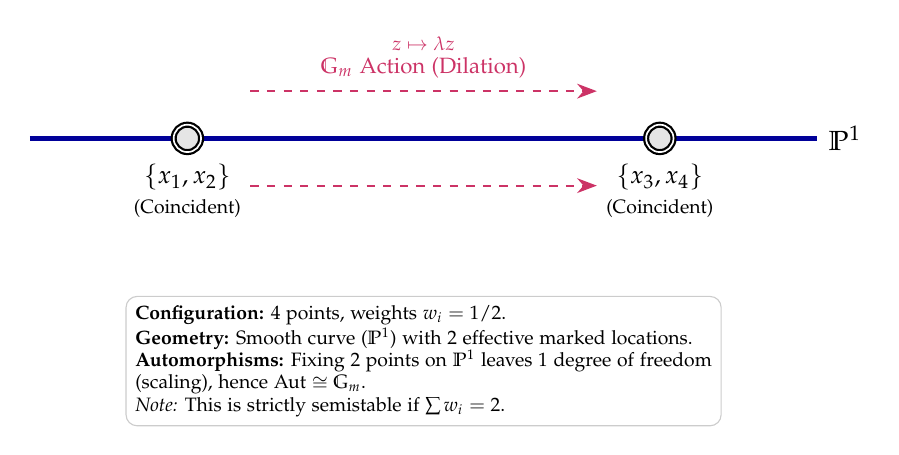
\begin{tikzpicture}[scale=2]
    % --- Definitions ---
    % The line (P^1)
    \coordinate (left_end) at (-2.5, 0);
    \coordinate (right_end) at (2.5, 0);
    
    % The two distinct locations for the coincident pairs
    \coordinate (loc1) at (-1.5, 0);
    \coordinate (loc2) at (1.5, 0);

    % --- Styles ---
    \tikzstyle{curve_line}=[ultra thick, color=blue!60!black]
    % Coincident Pair style (Weight 1 total)
    \tikzstyle{pair_point}=[
        draw=black, 
        double, 
        circle, 
        fill=gray!20, 
        inner sep=3.5pt, 
        thick
    ]
    % Flow arrows for Gm action
    \tikzstyle{flow_arrow}=[
        ->, 
        >={Stealth[length=2.5mm]}, 
        color=purple!80, 
        thick, 
        dashed
    ]

    % --- 1. Draw the Smooth Curve (Line) ---
    \draw[curve_line] (left_end) -- (right_end) node[right, color=black] {$\mathbb{P}^1$};

    % --- 2. Draw the Automorphism "Flow" ---
    % Since the automorphism is scaling (z -> \lambda z), we visualize it
    % as a flow moving away from one point and towards the other.
    \draw[flow_arrow] (-1.1, 0.3) -- (1.1, 0.3);
    \draw[flow_arrow] (-1.1, -0.3) -- (1.1, -0.3);
    
    \node[color=purple!80, font=\footnotesize] at (0, 0.45) {$\mathbb{G}_m$ Action (Dilation)};
    \node[color=purple!80, font=\scriptsize] at (0, 0.6) {$z \mapsto \lambda z$};


    % --- 3. Draw the Marked Points ---
    
    % Location 1: Pair {x1, x2} (e.g., at z=0)
    \node[pair_point] at (loc1) {};
    \node[below=0.2cm, align=center, font=\small] at (loc1) {
        $\{x_1, x_2\}$ \\ 
        \scriptsize (Coincident)
    };

    % Location 2: Pair {x3, x4} (e.g., at z=\infty)
    \node[pair_point] at (loc2) {};
    \node[below=0.2cm, align=center, font=\small] at (loc2) {
        $\{x_3, x_4\}$ \\ 
        \scriptsize (Coincident)
    };

    % --- 4. Annotations ---
    \node[draw=gray!40, fill=white, rounded corners, align=left, font=\scriptsize, anchor=north] at (0, -1) {
        \textbf{Configuration:} 4 points, weights $w_i=1/2$. \\
        \textbf{Geometry:} Smooth curve ($\mathbb{P}^1$) with 2 effective marked locations. \\
        \textbf{Automorphisms:} Fixing 2 points on $\mathbb{P}^1$ leaves 1 degree of freedom \\
        (scaling), hence Aut $\cong \mathbb{G}_m$. \\
        \textit{Note:} This is strictly semistable if $\sum w_i = 2$.
    };

\end{tikzpicture}
    \end{center}
    \caption{A strictly semistable object in \(\ol{M}_{0, \frac{1}{2}}^*\). }%
    \label{fig:semistablecurve}
    \end{figure}
\end{exm}

The Hassett moduli spaces have a wall-and chamber-structure, where for example, if $A = (\alpha, \ldots, \alpha)$ is $S_n$-symmetric, then $\ol{M}_{0,A}$ is constant for $\alpha \in \ab(\frac{1}{k+1}, \frac{1}{k})$, but on the walls we only have $\ol{M}_{0, A}^*$. The main observation is that if we write $\ol{M}_{0, \alpha}$ for $\ol{M}_{0, (\alpha, \ldots, \alpha)}$, then there are open immersions
\[ \ol{M}_{0, \frac{1}{k}-\ep} \subset \ol{M}_{0, \frac{1}{k}}^* \supset \ol{M}_{0, \frac{1}{k}+\ep}. \]
If we consider the complement $\ol{M}_{0, \frac{1}{k}}^* \setminus \ol{M}_{0, \frac{1}{k}-\ep}$, then it consists of curves which contain an irreducible component which is a tree in the dual graph and contains $k$ marked points, so this part of the moduli space has a factor which describes the rest of the curve and one which is $[\A^{k-2}/\G_m]$. More precisely, we have
\[ \ol{M}_{0, \frac{1}{k}}^* \setminus \ol{M}_{0, \frac{1}{k}-\ep} = \ol{M}^*_{0, (1, \frac{1}{k}, \ldots, \frac{1}{k})} \times \ol{M}^*_{0, (1, \frac{1}{k}, \ldots, \frac{1}{k})} \]

This actually allows us to construct a test configuration, where if we have $\P^1 \times \A^1$ with a bunch of sections, we can blow up a point on the central fiber and then contract the central $(-1)$-curve with all of the sections.

\begin{exer}
    Figure out what $\ol{M}_{0, \frac{1}{k}}^* \setminus \ol{M}_{0, \frac{1}{k}+\ep}$ is.
\end{exer}

For now, we will denote this picture by $\mc{M}^- \subset \mc{M} \supset \mc{M}^+$. Then in fact we actually have
\[ \mc{M} \setminus \mc{M}^+ = \ol{M}_{0, (1, \frac{1}{k}, \ldots, \frac{1}{k})} \times [\C/\C^{\times}], \]
where the second factor comes from the place where $k$ of the sections collide. In this picture, we can degenerate out a new rational tail which has only the $k$ colliding sections (which has a $\C^{\times}$-action), which is another example of a test configuration, as in~\Cref{fig:bubble}.

\begin{figure}[htpb]
\begin{center}
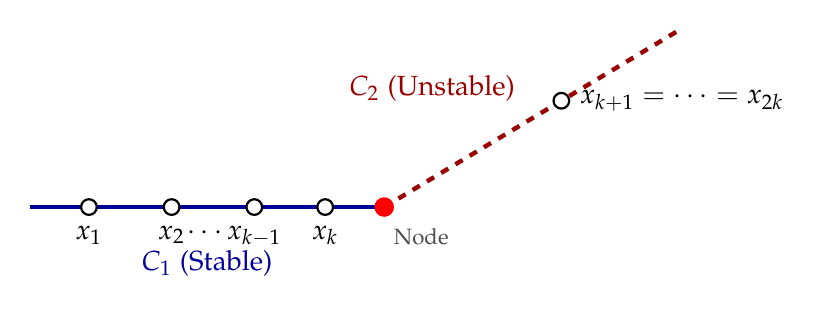
\begin{tikzpicture}[scale=1.5]
    % --- Styles ---
    \tikzstyle{component}=[ultra thick, color=blue!60!black]
    \tikzstyle{unstable_component}=[ultra thick, color=red!60!black, dashed]
    \tikzstyle{markpoint}=[draw=black, circle, fill=white, inner sep=2pt, thick]
    \tikzstyle{node_singularity}=[fill=red, circle, inner sep=2.5pt]
    \tikzstyle{label_text}=[font=\footnotesize, color=black!70]
    \tikzstyle{anno_box}=[draw=gray!30, fill=white, rounded corners, align=left, font=\scriptsize]

    % --- 1. Draw Components ---
    
    % Component 1 (Stable): Holds 4 points
    % Drawn horizontally
    \draw[component] (-3, 0) -- (0, 0) node[midway, below=0.4cm, color=blue!60!black] {$C_1$ (Stable)};
    
    % Component 2 (Unstable): Holds 1 point
    % Drawn at an angle to suggest it's "bubbling" or distinct
    % Dashed line indicates it is the unstable/contractible part
    \draw[unstable_component] (0, 0) -- (2.5, 1.5) node[midway, above left=0.1cm, color=red!60!black] {$C_2$ (Unstable)};

    % --- 2. Draw The Singularity ---
    \node[node_singularity] at (0, 0) {};
    \node[label_text, below right] at (0, -0.1) {Node};

    % --- 3. Draw Marked Points ---
    
    % Points on C_1 (x1 to x4)
    \node[markpoint, label=below:$x_1$] at (-2.5, 0) {};
    \node[markpoint, label=below:$x_2$] at (-1.8, 0) {};
    \node[label=below:$\cdots$] at (-1.5, 0) {};
    \node[markpoint, label=below:$x_{k-1}$] at (-1.1, 0) {};
    \node[markpoint, label=below:$x_{k}$] at (-0.5, 0) {};

    % Point on C_2 (x5)
    \node[markpoint, label=right:{$x_{k+1}=\cdots=x_{2k}$}] at (1.5, 0.9) {};

    % --- 4. Annotations ---
\end{tikzpicture}
\end{center}
\caption{A curve that we bubble out}%
\label{fig:bubble}
\end{figure}


Later, when we discuss good moduli spaces, there is a diagram
\begin{equation*}
\begin{tikzcd}
    \mc{M}^+ \ar[hookrightarrow]{r} \ar{d} & \mc{M} \ar{d} \ar[hookleftarrow]{r} &  \mc{M}^-  \ar{d} \\
    M^+ \ar{r} & M & M^- \ar{l}{\sim},
\end{tikzcd}
\end{equation*}
where the rightward arrow in the bottom row is a divisorial contraction.

In fact, there is a series of divisorial contractions
\[ \ol{M}_{0, n} \to \cdots \to \ol{M}_{0, A} \to \cdots \to (\P^1)^n \sslash \on{PGL}(2) \]
and another series of divisorial contractions
\[ \ol{M}_{0, n} \to \cdots \to \ol{M}_{0, A} \to \cdots \to \P^{n-3}. \]


\subsection{Divisors on $\ol{M}_{0,n}$}%
\label{sub:Divisors on m0nbar}

There are boundary divisors $\Delta_{I, J}$ where $I \sqcup J = \ab\{1, \ldots, n \}$ where the curve degenerates into two components, one with the markings from $I$ and the other with the markings from $J$. It is clear that
\[ \Delta_{I, J} \simeq \ol{M}_{0, \abs{I}+1} \times \ol{M}_{0, \abs{J}+1}. \]
We will denote their union by $\Delta$ and call it the total boundary.

It is easy to see that $\ol{M}_{0,n} \setminus \Delta \eqqcolon M_{0,n}$ consists only of smooth curves and is given by
\[ M_{0,n} = (\C^{\times} \setminus 1)^{n-3} \setminus \text{all diagonals}. \]
This has no Picard group, so the entire Picard group of $\ol{M}_{0,n}$ is generated by the boundary divisors. For example, $\ol{M}_{0,3}$ is a point, $\ol{M}_{0,4} = \P^1$, and $\ol{M}_{0,5}$ is $\P^1 \times \P^1$ blown up at three points.

\begin{exer}
    Compute the Picard rank of $\ol{M}_{0,n}$.
\end{exer}

If we consider a $1$-dimensional base $B$, then basic the theory of surfaces tells us that $\psi_{i|_B} = -\sigma_i^2$, and if we blow down all rational tails in $\mc{C}$ to form a new $\P^1$-bundle $\mc{D} \to B$ which has a section $\sigma_1$ with self-intersection $-r$ and a number of other sections $\tilde{\sigma}_i$ with self-intersection $+r$. If we now blow up the other collision points, then we see that
\[ (\psi_1 + \psi_i )_{|B}= \sum_{\substack{1 \in I \\ i \in J}} \Delta_{I \sqcup J} \cdot B. \]
In particular, because $\ol{M}_{0,n}$ is smooth, we have derived Keel's relation, which is that for all $i \neq j$, then
\[ \psi_i + \psi_j \sim \sum_{\substack{i \in I \\ j \in J}} \Delta_{I \sqcup J}. \]
These in fact generate all relations.

We now consider the morphism $f_{n+1} \colon \ol{M}_{0, n+1} \to \ol{M}_{0, n}$ given by deleting the last marked point and stabilizing. This is in fact the universal family over $\ol{M}_{0, n}$, so in particular it has $n$ disjoint sections $\sigma_1, \ldots, \sigma_n$. From this perspective, we can construct $\ol{M}_{0, 5}$ by blowing up the points on $\P^1 \times \P^1$ where the diagonal intersects the three horizontal sections corresponding to $0$, $1$, and $\infty$. If we blow down the four $(-1)$-curves corresponding to the diagonal section and the three fibers that we blew up, the family becomes the pencil of conics passing through four points on $\P^2$ and the reducible fibers are in fact the three degenerate members. In particular, we see that $\Pic(\ol{M}_{0,5}) = \Z^5$.

Another way to see this is to consider the sequence
\[ \ol{M}_{0,n} \simeq \ol{M}_{0, (\frac{1}{2}, \ldots, \frac{1}{2})} \to \ol{M}_{0, (\frac{1}{3}, \ldots, \frac{1}{3})} \to \cdots \to (\P^1)^n \sslash \on{PGL}(2) \]
and use this to compute the Picard rank, which is
\[ \rho(\ol{M}_{0,n}) = 2^{n-1} - \binom{n}{2} - 1. \]
A more precise description is that
\[ \Pic (\ol{M}_{0,n}) = \Z \ab<\Delta_{I \sqcup J}, \psi_1, \ldots, \psi_n> / \text{Keel}. \]
The blowup construction (really the one that starts with $\P^{n-3}$) proves that the Picard group also has no torsion.

One way to find a basis for the Picard group is the following. We will call $\Delta_{I \sqcup J}$ \textit{non-adjacent} if $I$ is not an arc when we arrange $1, \ldots, n$ in a circle.

\begin{prop}
    Non-adjacent boundary divisors form a basis of $\Pic(\ol{M}_{g,n})$.
\end{prop}

\begin{proof}
    We use Keel's relations to rewrite every divisor as a linear combination of non-adjacent ones, and then we check that the number of non-adjacent ones is exactly the Picard rank. 

    For example, if we have $I = \ab\{1, 2\}$, we will use the relations for $\psi_1 + \psi_2$, $\psi_3 + \psi_n$ (with a plus sign), $\psi_1 + \psi_n$, and $\psi_2 + \psi_3$ (with a minus sign), then the left hand side vanishes while the only adjacent boundary divisor remaining is the one with $I = \ab\{1,2\}$. The general case of this is left as an exercise, as is counting the non-adjacent boundary divisors.
\end{proof}

We have discussed the fact that $\ol{M}_{0,n}$ is a projective variety. We know it is proper, but we would like to produce an ample line bundle. One candidate is
\[ \psi - \Delta \coloneqq \psi_1 + \cdots + \psi_n - \sum {\Delta_{I \sqcup J}}. \]
The first step to proving that this is ample is to sum all of Keel's relations, which gives us
\[ (n-1)\psi = \abs{I} \abs{J} \Delta_{I \sqcup J}. \]
Because $\abs{I} \abs{J} \geq 2(n-2) > n-1$ (here $n \geq 4$), we see that
\[ \Psi - \Delta = \sum c_{I \sqcup J} \Delta_{I \sqcup J}, \]
where all coefficients are positive. 

We will now use the ampleness criterion and show that $(\psi - \Delta).B > 0$ for any irreducible proper curve $B \hookrightarrow \ol{M}_{0,n}$. If $B$ intersects the interior nontrivially, then by definition it has to intersect the boundary with positive degree. The other case is when $B \hookrightarrow \Delta_{I \sqcup J}$ lives inside one of the boundary divisors.

In this case, we have
\[ B \hookrightarrow \Delta_{I \sqcup J} \simeq \ol{M}_{0, k+1} \times \ol{M}_{0, n-k+1}. \]
Restricting $\psi - \Delta$, we obtain
\[ (\psi - \Delta)_{|\Delta_{I \sqcup J}} \simeq (\psi - \Delta)_{\ol{M}_{0, k+1}} \boxtimes (\psi -\Delta)_{\ol{M}_{0, n-k+1}}, \]
so we induct using the fact that on $\ol{M}_{0,4} \simeq \P^1$, $\psi - \Delta = \mc{O}(1)$.



\end{document}

%%% Local Variables:
%%% mode: latex
%%% TeX-master: t
%%% End:
